%\algrenewcommand\algorithmicprocedure{\textbf{}}
%\begin{algorithm}\small
%\caption{Modified Yao Step}\label{MYS}
%\begin{algorithmic}[0]
%\Statex \textbf{Input:} planar, t-spanner $G $; integer $k\geq 14 $
%\Statex \textbf{Output:} planar, t-spanner $G' $ with constant node degree
%
%\Statex
%
%\For{each node $p\in G $}
%	\State Define $k $ disjoint cones of size $2\pi/k $ around $p $.
%	\State Select for each non empty cone the shortest edge.
%	\For{each maximal sequence $s $ of empty cones}
%		\If{$|s|==1 $}
%			\State Let $nx $ and $ny $ be the incident edges on $p $ clockwise and \State counterclockwise, respectively, from the emtpy cone.
%			\If{either $nx $ or $ny $ has already been selected}
%				\State select the other edge
%				\Else
%				\State Select the shorter edge
%			\EndIf 
%		\Else
%			\State select the first $\lfloor \frac{|s|}{2} \rfloor $ unselected edges incident on $n $ clockwise from $s $
%			\State select the first $\lceil \frac{|s|}{2} \rceil $ unselected edges incident on $n $ counterclockwise from $s $
%		\EndIf
%	\EndFor
%\EndFor
%\State $ G' $ is the subgraph of $G $ consisting of all nodes which are in $G $ and all edges which fulfil that both endpoints of this edge have selected it. 
%\end{algorithmic}
%\end{algorithm}
\section{Algorithm}
This chapter introduces the \emph{reactive Modified Yao Step (RMYS)} and explains its functionality.
For the sake of completeness follows a scheme of the Modified Yao Step taken from \cite{kanj} and how this can be changed to a reactive approach.
In addition, there is an explanation of how RMYS operates.
Then there is a proof of correctness, followed by an brief analysis of the message complexity and message size of RMYS.
Afterwards, we see which properties the graph produced by RMYS obtains and which not.

\algrenewcommand\algorithmicprocedure{\textbf{}}
\begin{algorithm}\small
\caption{Modified Yao Step}\label{MYS}
\begin{algorithmic}[1]
\Statex \textbf{Input:} planar, connected graph $G $; integer $k\geq 14 $
\Statex \textbf{Output:} planar, connected graph $G' $ with constant node degree of at most $k $

\Statex

\For{each node $p\in G $}
	\State Define $k $ disjoint cones of size $2\pi/k $ around $p $.
	\State Select for each non empty cone the shortest edge.
	\For{each maximal sequence $s $ of empty cones}
		\If{$|s|==1 $}
			\State Let $nx $ and $ny $ be the incident edges on $p $ clockwise and \State counterclockwise, respectively, from the emtpy cone.
			\If{either $nx $ or $ny $ has already been selected}
				\State select the other edge
				\Else
				\State Select the shorter edge
			\EndIf 
		\Else
			\State select the first $\lfloor \frac{|s|}{2} \rfloor $unselected edges incident on $n $ clockwise from $s $
			\State select the first $\lceil \frac{|s|}{2} \rceil $unselected edges incident on $n $ counterclockwise from $s $
		\EndIf
	\EndFor
\EndFor
\Statex $ G' $ is the subgraph of $G $ consisting of all nodes which are in $G $ and all edges which fulfil that both endpoints of this edge have selected it. 
\end{algorithmic}
\end{algorithm}
 
Algorithm \ref{MYS} does not tell, in particular, how this can be computed on a node.
However, my reactive approach, called rMYS, is the following: Since every node knows its PDT-neighborhood (refer to algorithm \ref{RMYS}) which is used by the Modified Yao Step, it can execute this algorithm from line 1 to 14 without further knowledge about its neighborhood and hence, does not need to send any messages at all.
My approach of RMYS needs to send a RTS-message to each possible neighbor which send a message back if they did not select this edge.
This ensures that only bidirectional edges are used.
Since in most cases the edges are bidirectional a node sends only a so called protestmessage if it did not select an edge and thus, protests against the selection of this edge.

The following algorithm is the definition of RMYS.
For clarity, notice that both acronyms RMYS and rMYS mean \grqq reactive Modified Yao Step\grqq, but former is the algorithm which consists of rPDT, the reactive version of PDT, and rMYS, the reactive way of applying the Modified Yao Step to a planar and connected graph described above.
 
%\textbf{\algrenewcommand\algorithmicprocedure{\textbf{}}
\begin{algorithm}\small
\caption{Reactive Modified Yao Step (RMYS)}\label{RMYS}
\begin{algorithmic}[0]
\Statex \textbf{Input:} any connected graph $G $; integer $k\geq 14 $
\Statex \textbf{Output:} planar, connected graph $G' $ with constant node degree of at most $k $

\Statex

\For{each node $p \in G $}
	\State create the PDT-Neighborhood of $p $ using rPDT
	\State apply rMYS to $p $ using PDT-graph
	\State let each neighbor of $p $ create its RMYS-neighbors and send a protest message if $p $ \indent is not among them causing $p $ to remove this edge
\EndFor 
\end{algorithmic}
\end{algorithm}

\begin{figure}[h!]
\centering
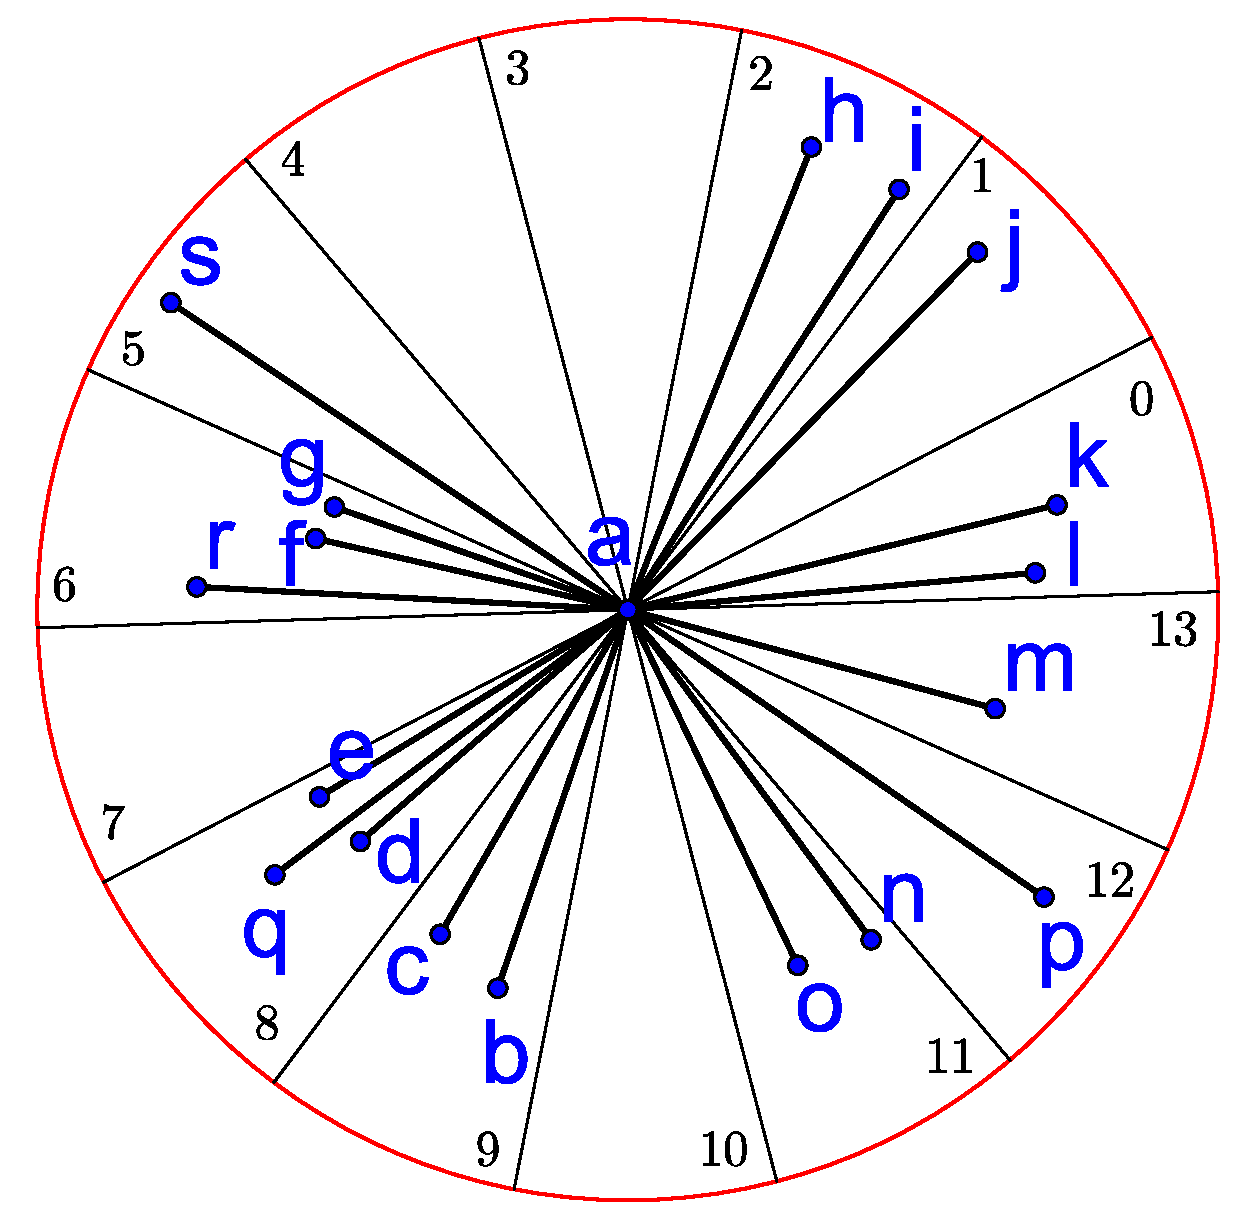
\includegraphics[width=0.6\linewidth]{eps/RMYS_1.eps}
\caption{An example graph and all edges drawn which are incident on $a $. The red circle shows the unit disk of $a $.}
\label{fig:RMYS_1}
\end{figure}

In the following RMYS is presented on the example given by figure \ref{fig:RMYS_1}.
Note that this example calculation is only performed on node $a $.
If one may want to create a complete graph, this algorithm must be executed for every node.

First, create the PDT neighborhood of $a $ using rPTD as explained in chapter \ref{PDT_section}.
Since nodes $p, q, r $ and $s $ are no PDT neighbors of $a $ and, hence they are not needed anymore, they are omitted in the following figures.
Now, the Modified Yao Step starts.
Place $k $ equally sized cones around $a $.
It does not matter where these cones start as long as they start at the same place for all nodes.
For the purpose of this example assume $k=14 $ and that the first cone starts at a horizontal line and runs counterclockwise.
The next step is that $a $ selects for each cone the shortest edge.
In figure \ref{fig:RMYS_2} these steps has been executed.
\begin{figure}[h!]
\centering
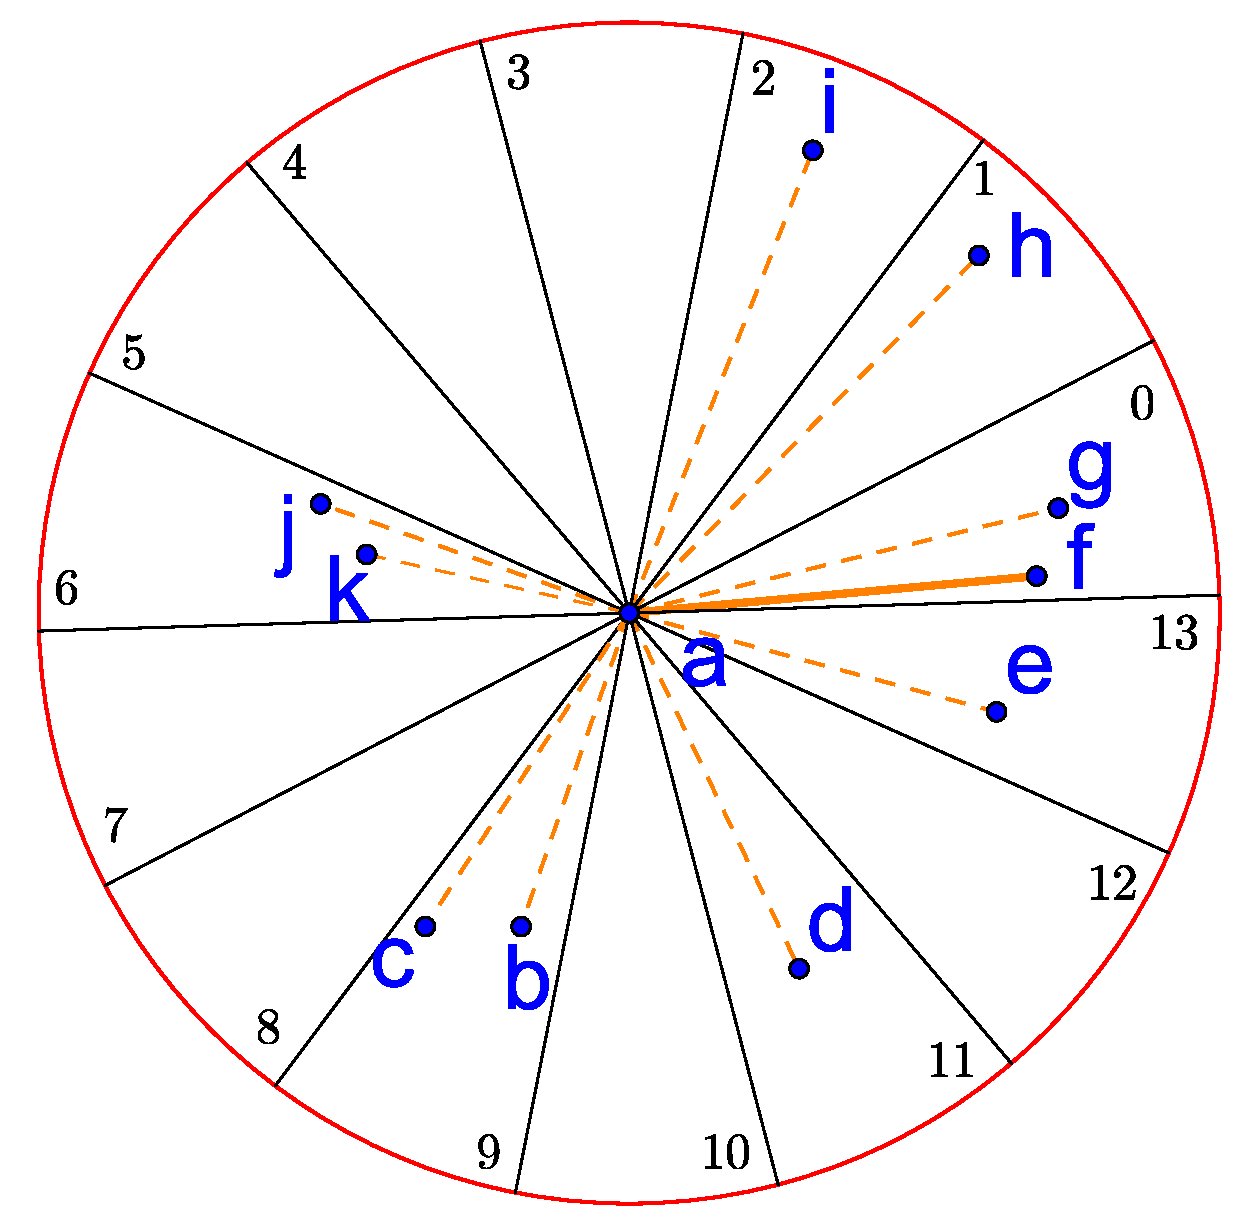
\includegraphics[width=0.6\linewidth]{eps/RMYS_2.eps}
\caption{An example graph with equally sized cones around $a $ and all edges drawn which are incident on $a $. All orange edges has been selected by reason of being the shortest edge in their cone.}
\label{fig:RMYS_2}
\end{figure}
Then, consider all maximal sequences of empty cones.
Let cones $3 $ to $5 $ be the first sequence to be considered.
Select the first $\lfloor \frac{|s|}{2} \rfloor = 1 $ unselected edges clockwise from $s $, with $s $ being the length of the sequence.
Hence, edge $ai $ is selected now.
Counterclockwise the next $\lceil \frac{|s|}{2} \rceil = 2$ unselected edges are selected.
For this reason edges $af $ and $ae $ are additionally selected.
The next empty sequence to analyze is cone 7.
In this case the next edge incident on $a $ clockwise and counterclockwise, respectively, from this cone has to be tested.
Since both edges $ae $ and $af $ are selected yet, no edge will be additionally added.
Moving on, the next empty sequence which is cone 10 must be inspected.
In this example $ao $ is already selected. 
However, $ab $ is not selected yet.
In order to fulfill the algorithm \ref{MYS} it selects $ab $ at this point in time.
The last sequence to analyze is cone 12.
For the same reason as in the sequence before $an $ gets selected.
The last step of the RMYS algorithm is that all of these selected neighbors test whether or not $a $ is also their neighbor.
If this is not the case for one node $z $, this edge is being deleted.
In this example every neighbor accepts $a $ as its neighbor.
Figure \ref{fig:RMYS_3} contains the final graph.

\begin{figure}[h!]
\centering
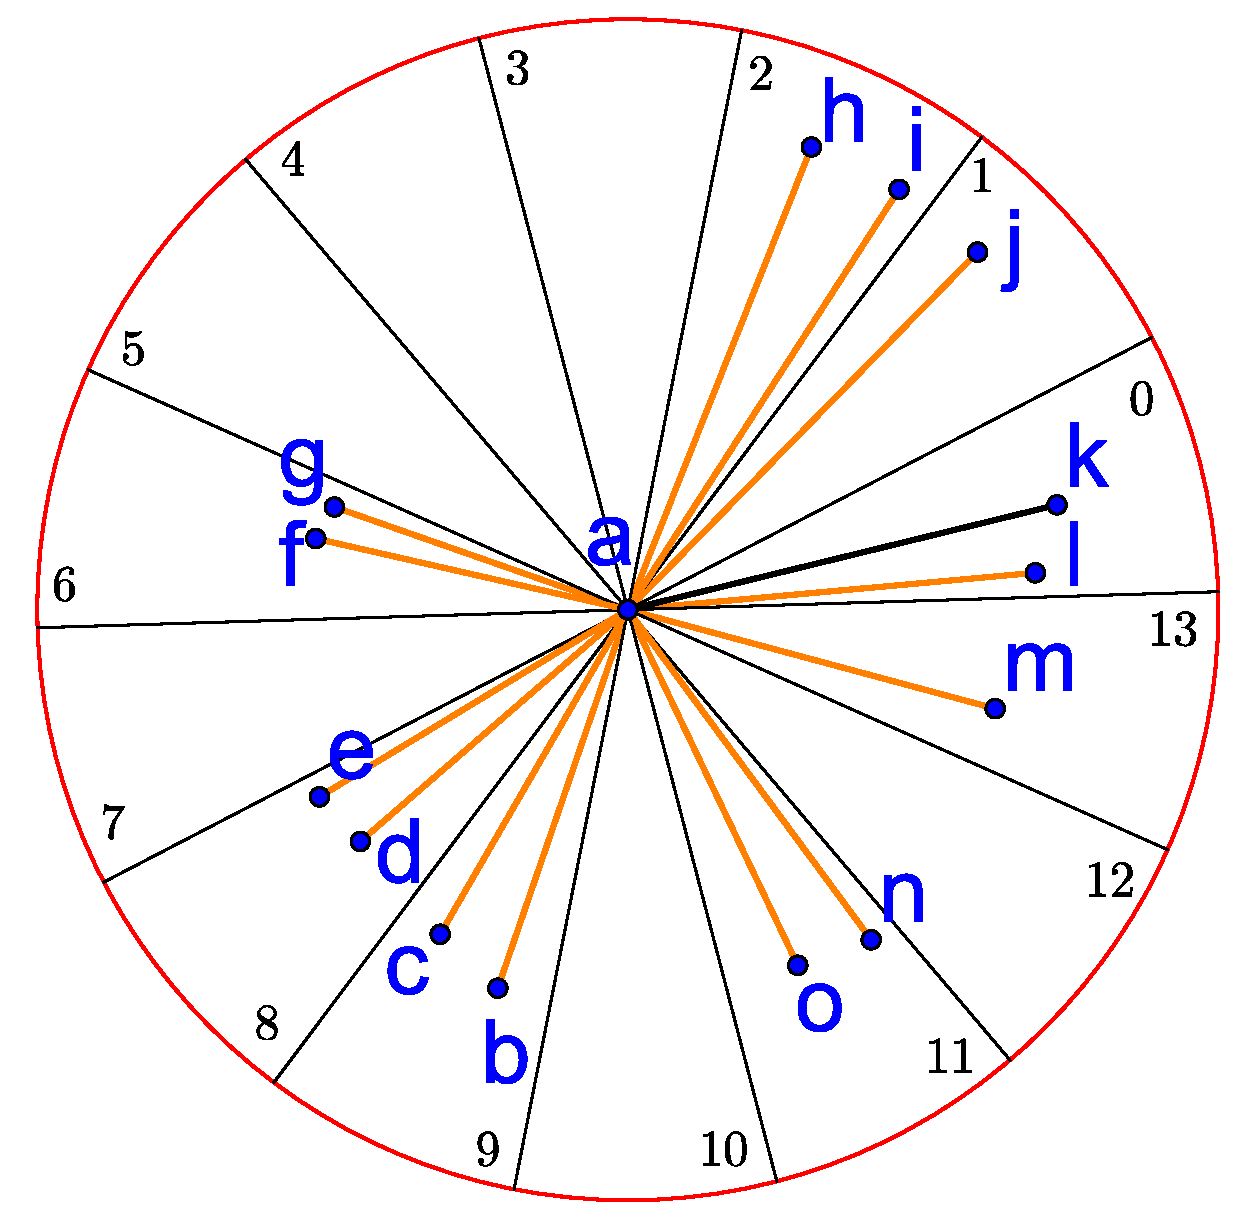
\includegraphics[width=0.6\linewidth]{eps/RMYS_3.eps}
\caption{This is the final graph with all edges drawn in orange which are incident on $a $ after the execution of RMYS.}
\label{fig:RMYS_3}
\end{figure}




\subsection{Proof of correctness}
\begin{proof}
\begin{equation*}
\begin{split}
	MYS(PDT) &\leftrightarrow RMYS\\
	MYS(PDT(v)) &\stackrel{a)}{\leftrightarrow} rMYS(rPDT(v)) \\
    MYS(PDT(v)) &\stackrel{b)}{\leftrightarrow} rMYS(PDT(v))\\
    MYS(PDT(v)) &\stackrel{c)}{\leftrightarrow} MYS(PDT(v)) 
\end{split}
\end{equation*}
We need to proof that the proposed reactive version of this algorithm is equal to a simple concatenation of first, the Partial Delaunay Triangulation and second, the Modified Yao Step on any node $v \in G$.
a) is the fragmentation of the proposition applied to a node $v $.
It is well known that $rPDT $ produces the same graph as the simple local approach, so b) holds true.
$rMYS $ does the same calculation as MYS right before the broadcast in the end.
Therefore, we need only to look at this broadcast.
The executing node $v $ sends a broadcast which must be overheard by all $PDT $ -Neighbors of $v $.
Because of the assumptions that every message arrives and arrives instantaneously, the message cannot get lost.
Every informed node checks whether or not it selects $v $ to be in its RMYS-Neighborhood.
If yes, it remains silent and otherwise it sends a protest message causing $v $ to remove this edge.
Hence, $v $ can check whether or not each node in it's neighborhood accepts this edge.
This leads to the same behavior MYS does and therefore, c) is true and completing this proof.
\end{proof}

\subsection{Message Complexity}
\label{message_complexity}
Let $N_{PDT}(u) $ be the message complexity of $PDT $ creating the neighborhood of Node $u \in G$.
First, $rPDT $ needs at most $n $ messages to create the $PDT $-neighborhood.
Next, the executing node sends at most $k $ messages to its neighbors to ask whether they accept their connection.
At most $k $ answers come back and therefore $k * 2 $.
Every one of this $k $ neighbors needs to calculate it's $PDT $-neighborhood and hence, $k*N_{PDT}(u) $.
The following equation put these reflections into one formula.
\begin{equation*}
\begin{split}
N_{RMYS}(u) &= \underbrace{N_{PDT}(u)}_{\theta (n)} +k *\underbrace{2}_{\theta (1)} + k*\underbrace{N_{PDT}(v)}_{\theta (n)} \\
\theta (N_{RMYS}(u)) &= \theta (n) 
\end{split}
\end{equation*}
Since $k $ is a constant it can be omitted in $O $-Notation.
The sum of the same complexity remains in the same complexity and hence, the message complexity of this algorithm is $\theta (n) $.

\subsection{Message Size}
If the assumption that every node has a unique position holds, this position can be used to identify each node uniquely.
Hence, two floats can be used to save this position resulting in a constant number of bits.
%Other information needed to send are only these node ids or a constant amount of it

\subsection{Properties of the RMYS-graph}
This section is devoted to the graph-properties the RMYS algorithms inherits.
First, it is important to know whether RMYS produces from any connected Unit Disk Graph a connected subgraph.
The first part of RMYS, the Partial Delaunay Triangulation, creates from a connected graph a connected subgraph.
Since rMYS removes edges it may be possible that the graph will be disconnected.
To analyze this we need to recognize that rMYS finds at least one edge per non empty cone.
Since these cones around a node $p $ cover the whole area around $p $ and if there is a node in it, there will be an edge for that cone. %PROOF !! vielleicht einfach
Hence, the graph cannot become disconnected. 

Following this, there is planarity.
The reactive approach of the Partial Delaunay Triangulation produces a planar graph and since the rMYS step of the RMYS-algorithm does not add any edges, the planarity property cannot be violated.
Hence, RMYS produces a planar graph.

Every node has a constant node degree of at most $k $.
First, for each cone the shortest edge is selected.
Resulting in $k $ edges if all cones are not empty.
For all other cases let $l $ be the total number of empty cones.
Then the first step selects $k-l $ edges in all non empty cones and at most $l $ edges are added in the second step.
This leads to a node degree of at most $k $.

